% This file was created by tikzplotlib v0.9.1.
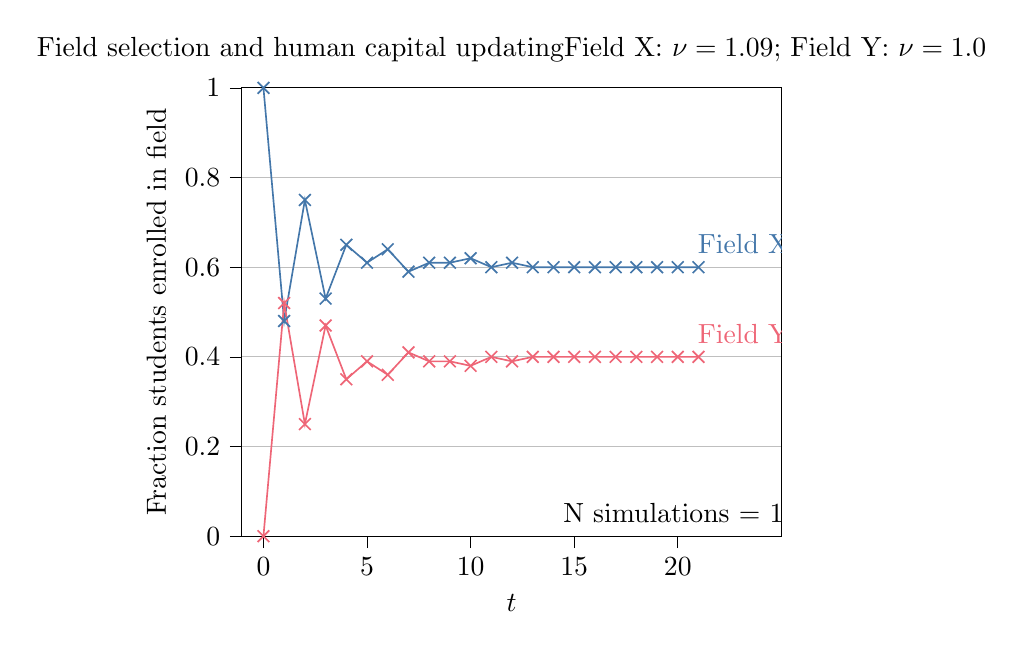
\begin{tikzpicture}

\definecolor{color0}{rgb}{0.266666666666667,0.466666666666667,0.666666666666667}
\definecolor{color1}{rgb}{0.933333333333333,0.4,0.466666666666667}

\begin{axis}[
height=207pt,
tick align=outside,
tick pos=left,
title={Field selection and human capital updating \\ Field X: \(\displaystyle \nu=1.09\); Field Y: \(\displaystyle \nu=1.0\)},
width=240pt,
x grid style={white!69.0196078431373!black},
xlabel={\(\displaystyle t\)},
xmin=-1.05, xmax=25,
xtick style={color=black},
xtick={0,5,10,15,20},
xticklabels={\(\displaystyle 0\),\(\displaystyle 5\),\(\displaystyle 10\),\(\displaystyle 15\),\(\displaystyle 20\)},
ylabel={Fraction students enrolled in field},
ymajorgrids,
ymin=0, ymax=1,
ytick style={color=black},
ytick={0,0.2,0.4,0.6,0.8,1},
yticklabels={\(\displaystyle 0\),\(\displaystyle 0.2\),\(\displaystyle 0.4\),\(\displaystyle 0.6\),\(\displaystyle 0.8\),\(\displaystyle 1\)}
]
\addplot [semithick, color0, mark=x, mark size=3, mark options={solid}]
table {%
0 1
1 0.48
2 0.75
3 0.53
4 0.65
5 0.61
6 0.64
7 0.59
8 0.61
9 0.61
10 0.62
11 0.6
12 0.61
13 0.6
14 0.6
15 0.6
16 0.6
17 0.6
18 0.6
19 0.6
20 0.6
21 0.6
};
\addplot [semithick, color1, mark=x, mark size=3, mark options={solid}]
table {%
0 0
1 0.52
2 0.25
3 0.47
4 0.35
5 0.39
6 0.36
7 0.41
8 0.39
9 0.39
10 0.38
11 0.4
12 0.39
13 0.4
14 0.4
15 0.4
16 0.4
17 0.4
18 0.4
19 0.4
20 0.4
21 0.4
};
\draw (axis cs:20.5,0.63) node[
  anchor=base west,
  text=color0,
  rotate=0.0
]{Field X};
\draw (axis cs:20.5,0.43) node[
  anchor=base west,
  text=color1,
  rotate=0.0
]{Field Y};
\draw (axis cs:14,0.03) node[
  anchor=base west,
  text=black,
  rotate=0.0
]{N simulations = 100};
\end{axis}

\end{tikzpicture}
